\chapter{Benchmarking}
	In section \ref{sec:privatecloud_cost} on page \pageref{sec:privatecloud_cost} it was argued that the cost of running a private cloud, has been drastically lowered by the introduction of low-powered devices such as the Raspberry Pi. In this section, the performance of running the implementation on a Raspberry Pi 1 Model B+, will be compared to that of a reference desktop machine, referred to as the Server. As such, this will \emph{not} be a traditional benchmark. The purpose of this section is \emph{not} to compare the implementation to \emph{other} existing systems, but to \emph{itself}.

	The devices used for this test are found on table \ref{tab:bench:devices} on page \pageref{tab:bench:devices}. The Client machine, is the device all tests are performed \emph{from}. These tests are done using the Apache Benchmark \emph{(ab)} tool\cite{ab_tool}. The complete output of \emph{all} tests performed for this chapter, are found in appendix \ref{appendix:benchmark}.

	The Rasbperry Pi 1 Model B+ and the Server machines, are used for hosting the back-end. On each of them, \emph{one} user is stored -- the admin user -- and \emph{one} password is stored. Each test will then perform $10.000$ requests, each \verb=GET='ing the password. The tests are run with with a concurrency level of 10 \emph{(i.e. 10 requests will be made at the same time)}, which is ab's default settings. Since caching is not enabled on the servers, no performance will be gained from requesting the same password over and over again.	

	\begin{table}[h!]
		\begin{tabularx}{\textwidth}{ R{0.3} | L{0.5} | L{0.2} }
			\textbf{Machine} 					& \textbf{CPU} 									& \textbf{RAM} 	\\
			\hline
			Raspberry Pi 1 B+  					& Broadcom BCM2835 @ 700 MHz  					& 512MB RAM 	\\
			Server 								& Intel Core i5-2400 @ 3.10GHz		& 8GB RAM 		\\
			Client 								& Intel Core i5-3570K @ 3.40GHz 		& 16GB RAM 		\\
		\end{tabularx}

		\caption{Devices used for the benchmarking.}
		\label{tab:bench:devices}
	\end{table}

	For these tests, it was chosen that the back-ends would be using the SQLite database. This choice was made, on the assumption that this would be the best option, for low-powered devices as argued in section \ref{sec:restrict:database} on page \pageref{sec:restrict:database}. The results of running these tests, are found on figure \ref{fig:bench:arch} on page \pageref{fig:bench:arch}. 

	As seen, the Raspberry Pi does not handle itself very well under pressure, compared to the Server. In fact, it is doing $~4.9$ times \emph{worse}. However, despite this \emph{horrible} benchmark, the implementation is \emph{usable} on the Raspberry Pi. However, the non-functional requirement \#\ref{requirement:delay} regarding maximum delay the user experiences, \emph{might} be violated, using this setup. Playing around with it, it \emph{does} feel sluggish, but this is easily mitigated by the use of a more powerful, newer, more power efficient, and -- most importantly -- equally cheap Raspberry Pi 3. But unfortunately it has not been possible to acquire a Raspberry Pi 3 for testing purposes, in time for this project.

	\begin{figure}[!h]
		\centering
	    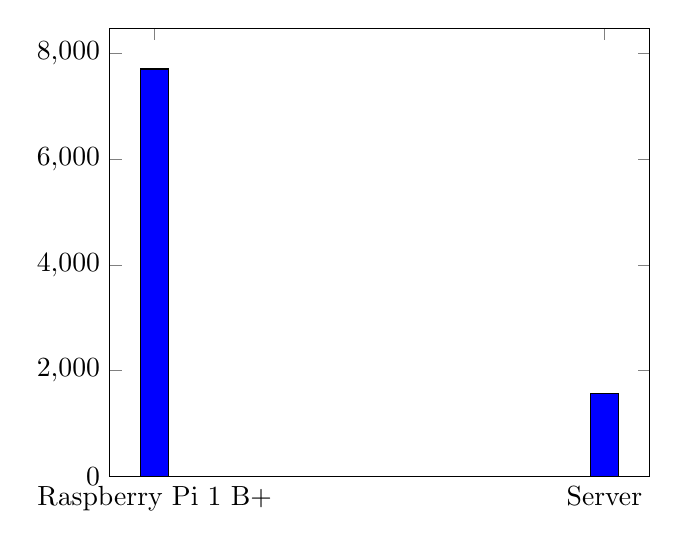
\begin{tikzpicture}
	        \begin{axis}[
	            symbolic x coords={Raspberry Pi 1 B+, Server},
	            xtick=data,
	            ymin=0
	          ]
	            \addplot[ybar,fill=blue] coordinates {
	                (Raspberry Pi 1 B+,  7704.454)
	                (Server, 1576.162)
	            };
	        \end{axis}
	    \end{tikzpicture}
	    \caption{Comparison of performance, between running the implementation on an RPI1B+ and a machine powered by an intel i5-2400 processor. An SQLite database is used. Lower is better.}
	    \label{fig:bench:arch}
	\end{figure}

	However, even the performance of the reference server, seems extremely sub-par. As such, a benchmark is run, comparing the various database technologies: SQLite, MySQL, and Postgres. The results of these tests are found on figure \ref{fig:bench:db} on page \pageref{fig:bench:db}. As it is seen SQLite is \emph{several magnitudes} slower than both MySQL and Postgres -- around a factor of $12$.

	This is, however, to be expected. Both MySQL and Postgres are designed to be performance databases, whereas SQLite is designed to have a minimal impact and run without a separate service. As such, even though the SQLite might result in a \emph{horrible} performance, compared to the other two, it could still potentially be beneficial to run on low-powered devices.

	\begin{figure}[!h]
		\centering
	    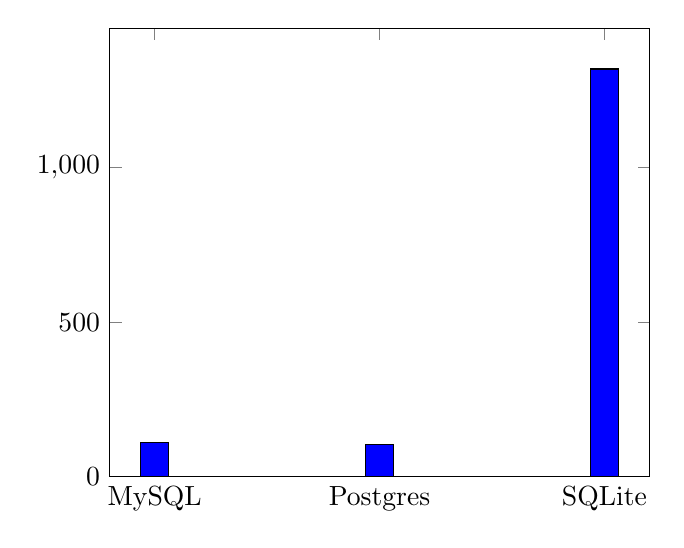
\begin{tikzpicture}
	        \begin{axis}[
	            symbolic x coords={MySQL, Postgres, SQLite},
	            xtick=data,
	            ymin=0
	          ]
	            \addplot[ybar,fill=blue] coordinates {
	                (MySQL,  109.739)
	                (Postgres, 102.792)
	                (SQLite,   1319.779)
	            };
	        \end{axis}
	    \end{tikzpicture}
	    \caption{Comparison of performance, of MySQL, Postgres, and SQLite database systems. Results are achieved by performing 10.000 requests, with a concurrency level of 10. Lower is better.}
	    \label{fig:bench:db}
	\end{figure}

	A final experiment is made to determine this assumption. This is done by installing and running the \verb=mysql-server= on the Raspberry Pi. The exact same test as before is performed and the results of this test is seen on figure \ref{fig:bench:rpi-bench} on page \pageref{fig:bench:rpi-bench}. As it appears, the fundamental assumption of SQLite being superior on such low-powered devices is actually \emph{wrong}. It would even seem that the MySQL database is \emph{slightly} faster. However, this could also just be due to variations. As such, performance-wise, SQLite really has no place being used as a database. However, there is more than just performance to the selection. Where initializing the system using a MySQL database is slightly cumbersome, a SQLite database takes virtually no work. As such, for setups favouring simplicity instead of performance, SQLite is still the go-to database, despite its horrible performance.

	\begin{figure}[!h]
		\centering
	    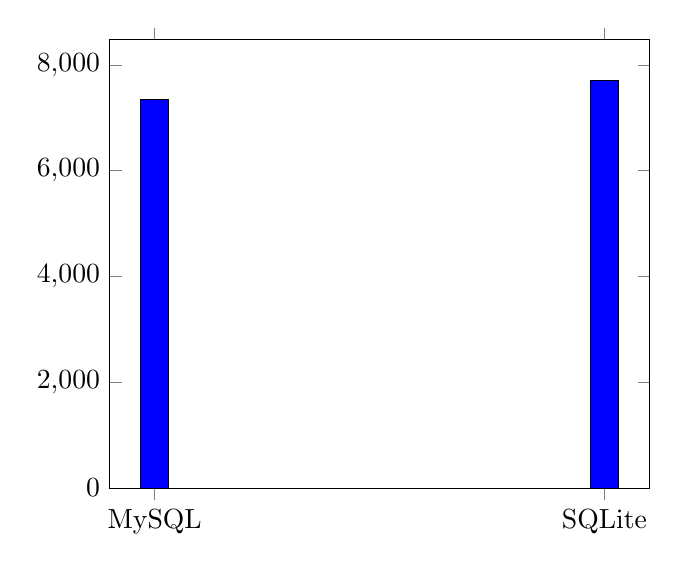
\begin{tikzpicture}
	        \begin{axis}[
	        	ybar,
	            symbolic x coords={MySQL, SQLite},
	            xtick=data,
	            ymin=0
	            %ytick={0,1000,2000,3000,4000,5000,6000,7000}
	          ]
	            \addplot[ybar,fill=blue] coordinates {
	                (MySQL,  7349.056)
	                (SQLite,   7704.454)
	            };
	        \end{axis}
	    \end{tikzpicture}
	    \caption{Comparing performance of a SQLite ands a MySQL database on the Raspberry Pi. Lower is better.}
	    \label{fig:bench:rpi-bench}
	\end{figure}


	\section{Final Remarks}
		Admittedly, the scientific-process of these benchmarks have been less than ideal. Many factors could effectively influence these tests greatly, such as the amount of \emph{other} traffic on the network at the time of the test, or the quality of the SD card that the Pi is equipped with. However, the intent of this chapter was not to adhere to the highest possible scientific standards, but more as a way of determining the viability of running the implementation on a Raspberry Pi. As such, it is finally concluded, that while running it on a Model 1 B+ is sluggish, it is still \emph{usable} for individuals.